% Options for packages loaded elsewhere
\PassOptionsToPackage{unicode}{hyperref}
\PassOptionsToPackage{hyphens}{url}
%
\documentclass[
]{article}
\usepackage{amsmath,amssymb}
\usepackage{lmodern}
\usepackage{iftex}
\ifPDFTeX
  \usepackage[T1]{fontenc}
  \usepackage[utf8]{inputenc}
  \usepackage{textcomp} % provide euro and other symbols
\else % if luatex or xetex
  \usepackage{unicode-math}
  \defaultfontfeatures{Scale=MatchLowercase}
  \defaultfontfeatures[\rmfamily]{Ligatures=TeX,Scale=1}
\fi
% Use upquote if available, for straight quotes in verbatim environments
\IfFileExists{upquote.sty}{\usepackage{upquote}}{}
\IfFileExists{microtype.sty}{% use microtype if available
  \usepackage[]{microtype}
  \UseMicrotypeSet[protrusion]{basicmath} % disable protrusion for tt fonts
}{}
\makeatletter
\@ifundefined{KOMAClassName}{% if non-KOMA class
  \IfFileExists{parskip.sty}{%
    \usepackage{parskip}
  }{% else
    \setlength{\parindent}{0pt}
    \setlength{\parskip}{6pt plus 2pt minus 1pt}}
}{% if KOMA class
  \KOMAoptions{parskip=half}}
\makeatother
\usepackage{xcolor}
\usepackage[margin=1in]{geometry}
\usepackage{longtable,booktabs,array}
\usepackage{calc} % for calculating minipage widths
% Correct order of tables after \paragraph or \subparagraph
\usepackage{etoolbox}
\makeatletter
\patchcmd\longtable{\par}{\if@noskipsec\mbox{}\fi\par}{}{}
\makeatother
% Allow footnotes in longtable head/foot
\IfFileExists{footnotehyper.sty}{\usepackage{footnotehyper}}{\usepackage{footnote}}
\makesavenoteenv{longtable}
\usepackage{graphicx}
\makeatletter
\def\maxwidth{\ifdim\Gin@nat@width>\linewidth\linewidth\else\Gin@nat@width\fi}
\def\maxheight{\ifdim\Gin@nat@height>\textheight\textheight\else\Gin@nat@height\fi}
\makeatother
% Scale images if necessary, so that they will not overflow the page
% margins by default, and it is still possible to overwrite the defaults
% using explicit options in \includegraphics[width, height, ...]{}
\setkeys{Gin}{width=\maxwidth,height=\maxheight,keepaspectratio}
% Set default figure placement to htbp
\makeatletter
\def\fps@figure{htbp}
\makeatother
\setlength{\emergencystretch}{3em} % prevent overfull lines
\providecommand{\tightlist}{%
  \setlength{\itemsep}{0pt}\setlength{\parskip}{0pt}}
\setcounter{secnumdepth}{5}
\ifLuaTeX
  \usepackage{selnolig}  % disable illegal ligatures
\fi
\IfFileExists{bookmark.sty}{\usepackage{bookmark}}{\usepackage{hyperref}}
\IfFileExists{xurl.sty}{\usepackage{xurl}}{} % add URL line breaks if available
\urlstyle{same} % disable monospaced font for URLs
\hypersetup{
  pdftitle={Comparing two or more means},
  pdfauthor={Furtado Jr, Ovande},
  hidelinks,
  pdfcreator={LaTeX via pandoc}}

\title{Comparing two or more means}
\author{\href{http://drfurtado.us}{Furtado Jr, Ovande}}
\date{Last updated on 2022-04-19}

\begin{document}
\maketitle

{
\setcounter{tocdepth}{2}
\tableofcontents
}
\begin{center}\rule{0.5\linewidth}{0.5pt}\end{center}

\hypertarget{one-way-anova}{%
\section{One-Way ANOVA}\label{one-way-anova}}

\hypertarget{readme}{%
\subsection{Readme}\label{readme}}

Other formats: \href{z-test.pdf}{PDF} \textbar{} \href{z-test.html}{HTML}

Hint: use Control+F (Windows) or Command+F (Mac) to search this page

\begin{center}\rule{0.5\linewidth}{0.5pt}\end{center}

\hypertarget{learning-objectives}{%
\subsection{Learning objectives}\label{learning-objectives}}

\begin{enumerate}
\def\labelenumi{\arabic{enumi}.}
\tightlist
\item
  Deciding when to use the z test
\item
\end{enumerate}

\hypertarget{when-to-use-it}{%
\subsection{When to use it?}\label{when-to-use-it}}

When you want to compare two or more sample means. In addition, there is a single quantitative (either interval or ratio) dependent variable and a single categorical independent variables with \(i\) independent groups ( \(i\geq 2\) ).

\hypertarget{stating-the-hypotheses}{%
\subsection{Stating the Hypotheses}\label{stating-the-hypotheses}}

\textbf{Null hypothesis}

\(H_0:\) There is no difference among the group means.

\(H_0:\mu_1 = \mu_2 = \ldots = \mu_i\)

where, \(\mu_1\) is the population mean for group 1; \(\mu_2\) is the population mean for group 2; \(\mu_i\) is the population mean for group \(i\).

\textbf{Alternative hypothesis}

\(H_a:\) At least one group differs significantly from the others.

\(H_a:\mu_1 \neq \mu_2 = \ldots \neq \mu_i\)

\begin{center}\rule{0.5\linewidth}{0.5pt}\end{center}

\hypertarget{assumptions}{%
\subsection{Assumptions}\label{assumptions}}

\begin{enumerate}
\def\labelenumi{\arabic{enumi}.}
\tightlist
\item
  data level - the DV should be measured at the continuous level (interval or ratio);
\item
  related groups - the IV should consist of at least two categorical, \texttt{independent} groups;
\item
  independence of observation - there is no relationship between the observations in each group or between the groups themselves;
\item
  normality: the DV should be approximately normally distributed for each category of the independent variable;
\item
  homogeneity of variance - homogeneity of variance: the standard deviation of the scores on the dependent variable are the same
\end{enumerate}

\hypertarget{test-statistic}{%
\subsection{Test statistic}\label{test-statistic}}

\[
F = \dfrac{\mbox{mean square between}}{\mbox{mean square error}}
\] where, \(MSb\) is represents the mean square between groups and \(MSw\) is the mean square within groups.

SSw = difference between each individual score ( \(Yik\) ) from their group mean ( \(\bar{Y}k\) )

SSb = difference between the group means ( \(\bar{Y}k\) ) and the grand mean ( \(\bar{Y}\) )

\begin{longtable}[]{@{}
  >{\raggedright\arraybackslash}p{(\columnwidth - 8\tabcolsep) * \real{0.2000}}
  >{\raggedright\arraybackslash}p{(\columnwidth - 8\tabcolsep) * \real{0.2000}}
  >{\raggedright\arraybackslash}p{(\columnwidth - 8\tabcolsep) * \real{0.2000}}
  >{\raggedright\arraybackslash}p{(\columnwidth - 8\tabcolsep) * \real{0.2000}}
  >{\raggedright\arraybackslash}p{(\columnwidth - 8\tabcolsep) * \real{0.2000}}@{}}
\caption{\label{tab:f-test} APA style ANOVA table}\tabularnewline
\toprule()
\begin{minipage}[b]{\linewidth}\raggedright
\end{minipage} & \begin{minipage}[b]{\linewidth}\raggedright
df
\end{minipage} & \begin{minipage}[b]{\linewidth}\raggedright
sum of squares
\end{minipage} & \begin{minipage}[b]{\linewidth}\raggedright
mean squares
\end{minipage} & \begin{minipage}[b]{\linewidth}\raggedright
\emph{F}-statistic
\end{minipage} \\
\midrule()
\endfirsthead
\toprule()
\begin{minipage}[b]{\linewidth}\raggedright
\end{minipage} & \begin{minipage}[b]{\linewidth}\raggedright
df
\end{minipage} & \begin{minipage}[b]{\linewidth}\raggedright
sum of squares
\end{minipage} & \begin{minipage}[b]{\linewidth}\raggedright
mean squares
\end{minipage} & \begin{minipage}[b]{\linewidth}\raggedright
\emph{F}-statistic
\end{minipage} \\
\midrule()
\endhead
between groups & \emph{df}\textsubscript{b} = G - 1 & \(                                                                                                                                                                                                                                                                                                                                                           
                                                                                                                                                                                                                                                                                                \displaystyle\sum_{k=1}^G N_k(\bar{Y}_k - \bar{Y})^2                                              
                                                                                                                                                                                                                                                                                                \) & MS\textsubscript{b} = SS\textsubscript{b} / \emph{df}\textsubscript{b} & F = MS\textsubscript{b} / MS\textsubscript{w} \\
within groups & \emph{df}\textsubscript{w} = N - G & \(                                                                                                                                                                                                                                                                                                                                                           
                                                                                                                                                                                                                                                                                                \displaystyle\sum_{k=1}^G \displaystyle\sum_{i = 1}^{N_k} ({Y}_{ik} - \bar{Y}_k)^2                
                                                                                                                                                                                                                                                                                                \) & MS\textsubscript{w} = SS\textsubscript{w} / \emph{df}\textsubscript{w} & \\
& & & & \\
\bottomrule()
\end{longtable}

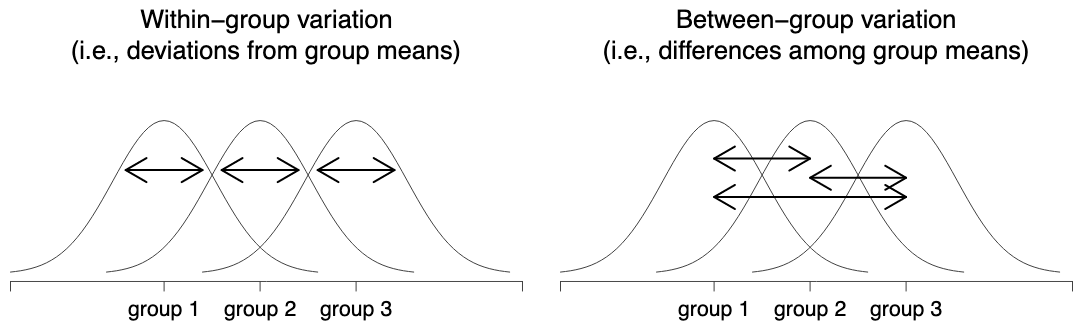
\includegraphics{images/paste-88B3A2B2.png}

\hypertarget{sampling-distribution}{%
\subsection{Sampling distribution}\label{sampling-distribution}}

When testing the null hypothesis with the \emph{F}-test, use the \href{https://statkat.com/sampling-distribution/anova/f-and-t.php}{sampling distribution of \emph{F} and \emph{t}}. The \emph{F} distribution is used to test if at least one sample mean is different from the others sample means. If the \emph{F} test is significant, further analyses must be performed to verify where the difference lies.

Assume we are comparing 3 sample means ( \(\bar{x_1}\), \(\bar{x_2}\), and \(\bar{x_3}\) ). There are three possible pairwise comparisons; e.g., 1x2, 1x3, and 2x3. The result of the F test only tell us if at least one of the pairwise comparisons is significant. It does not tell us which is which one(s) is(are) significant.

One needs to run t tests on each of the pairwise comparison to find out possible significant differences; this is referred as \texttt{post-hoc} analysis.

\hypertarget{significance}{%
\subsection{Significance}\label{significance}}

To find out whether the test is significant, compare the observed test statistics (\emph{F} value) with the critical value after considering the \textbf{alpha value}, the \textbf{type of test} (two-sided, right-sided, or left sided), and the \textbf{degrees of freedom}.

\begin{itemize}
\item
  compare the observed test statistic with the critical value

  \begin{itemize}
  \tightlist
  \item
    if the observed \emph{F} value is equal or greater than the critical value, reject the \(H_0\) ; or
  \end{itemize}
\item
  compare the observed \(p\) value\footnote{Value calculated by the statistical package; i.e., jamovi, SPSS or by using an online calculator such as \href{https://statkat.com/online-calculators/critical-f-value-given-alpha.php}{StatKat}.} with the alpha value (\$\textbackslash alpha\$).

  \begin{itemize}
  \tightlist
  \item
    if the calculate \(p\) value is less than the \(\alpha\), reject the \(H_0\)
  \end{itemize}
\end{itemize}

\textbf{Critical Value for} \(F\) \textbf{Statistic}

\[
F = \frac{k-1}{n-k}
\]

where:

\(F\) represents the F distribution.

\(k\) is the number of treatments (groups).

\(n\) is the total number of observations.

\begin{center}\rule{0.5\linewidth}{0.5pt}\end{center}

\hypertarget{confidence-interval-for-mu}{%
\subsection{\texorpdfstring{Confidence Interval for \(\mu\)}{Confidence Interval for \textbackslash mu}}\label{confidence-interval-for-mu}}

The confidence interval is typically reported along with the statistic (i.e.~mean, standard deviation, etc) when performing a significance test. However, it also be used as a \href{https://statkat.com/confidence-interval-as-test/one-sample-z-test.php}{significant test}.

Below is the equation used to calculate the CI for the difference in treatment means.

\[
(\bar{x}_{1} - \bar{x}_{2}) \pm t\sqrt{\text{MSE}\left(\frac{1}{n_{1}} + \frac{1}{n_{2}}\right)}
\]

where:

\(\bar{x}_{1}\) is the mean of the first sample.

\(\bar{x}_{2}\) is the mean of the second sample.

\(t\) refers to the \(t\) distribution with degrees of freedom equal to \(n-k\).

\(MSE\) is the mean square error term obtained from the ANOVA table \(\left[\frac{SSE}{n-k}\right]\)

\(n_{1}\) is the number of observations in the first sample.

\(n_{2}\) is the number of observations in the second sample.

\begin{center}\rule{0.5\linewidth}{0.5pt}\end{center}

\hypertarget{effect-size}{%
\subsection{Effect size}\label{effect-size}}

There's a different ways to measure the effect size in an ANOVA, but the most commonly used measures are \(\eta^2\) (\textbf{eta squared}) and partial \(\eta^2\). Since for a one-way analysis of variance they're identical, only the \(\eta^2\) is provided below. The definition of \(\eta^2\) is actually really simple. The values of \(SSb\) and \(SStot\) are taken from the the ANOVA table.

\[
\begin{align}
\eta^2 = R^2 
&= \dfrac{\mbox{sum of squares between}}{\mbox{sum of squares total}}
\end{align}
\]

One can also use the \(\omega^2\) (omega squared), which is arguably the unbiased estimate of the effect size when running the One-Way ANOVA. The equation of the \(\omega^2\) is provided below:

\[
\omega^2 = \frac{\mbox{sum of squares between} - \mbox{df between} \times \mbox{mean square error}}{\mbox{sum of squares total} + \mbox{mean square error}}
\]

\begin{center}\rule{0.5\linewidth}{0.5pt}\end{center}

\hypertarget{example}{%
\subsection{Example}\label{example}}

Is the fundamental movement skill total score on the FG-COMPASS\footnote{\url{http://fgcompass.com}} different between children from \texttt{low}, \texttt{moderate}, and \texttt{high} economic class?

\hypertarget{data3}{%
\subsubsection[Data]{\texorpdfstring{Data\footnote{This is a made-up data set.}}{Data}}\label{data3}}

Either type in the data below into your preferred statistical package or \href{data_les_1anova.csv}{click here} to download the csv file.

\begin{longtable}[]{@{}lll@{}}
\caption{(\#tab:data\_anova1) Fictitious data comprised of three independent groups.}\tabularnewline
\toprule()
\endhead
Low & Moderate & High \\
23 & 12 & 25 \\
33 & 16 & 34 \\
11 & 22 & 23 \\
22 & 15 & 33 \\
22 & 12 & 22 \\
\bottomrule()
\end{longtable}

\hypertarget{hypotheses}{%
\subsubsection{Hypotheses}\label{hypotheses}}

\(H_0:\) There is no difference among the \texttt{SES} group means.

\(H_0:\mu_1 = \mu_2 = \ldots = \mu_i\)

\(H_a:\) At least one \texttt{SES} group differs significantly from the others.

\(H_a:\mu_1 \neq \mu_2 = \ldots \neq \mu_i\)

\hypertarget{running-the-test}{%
\subsubsection{Running the test}\label{running-the-test}}

I demonstrate below how to test the \(H_0\) with the statistical package \texttt{jamovi}. We will use a two-sided test with an alpha level set to .05.

\hypertarget{jamovi}{%
\paragraph{jamovi}\label{jamovi}}

ANOVA \textgreater{} ANOVA

\begin{itemize}
\tightlist
\item
  Put your dependent (quantitative) variable in the box below \texttt{Dependent\ Variable} and your independent (grouping) variable in the box below \texttt{Fixed\ Factors}.
\end{itemize}

\hypertarget{output---descriptive-stats}{%
\subparagraph{Output - Descriptive stats}\label{output---descriptive-stats}}

\begin{verbatim}

 DESCRIPTIVES

 Descriptives                                      
 ───────────────────────────────────────────────── 
                          ses         fms scores   
 ───────────────────────────────────────────────── 
   N                      Low                  5   
                          Moderate             5   
                          High                 5   
   Mean                   Low           22.20000   
                          Moderate      15.40000   
                          High          27.40000   
   Standard deviation     Low           7.791020   
                          Moderate      4.098780   
                          High          5.683309   
   Skewness               Low         -0.1275071   
                          Moderate      1.264894   
                          High         0.4690286   
   Std. error skewness    Low          0.9128709   
                          Moderate     0.9128709   
                          High         0.9128709   
   Kurtosis               Low           1.954056   
                          Moderate      1.588010   
                          High         -3.040669   
   Std. error kurtosis    Low           2.000000   
                          Moderate      2.000000   
                          High          2.000000   
   Shapiro-Wilk W         Low          0.9098903   
                          Moderate     0.8622023   
                          High         0.8354254   
   Shapiro-Wilk p         Low          0.4669314   
                          Moderate     0.2362639   
                          High         0.1526686   
 ───────────────────────────────────────────────── 
\end{verbatim}

\hypertarget{output---overall-test}{%
\subparagraph{Output - Overall test}\label{output---overall-test}}

\begin{verbatim}

 ANOVA

 ANOVA - fms scores                                                                         
 ────────────────────────────────────────────────────────────────────────────────────────── 
                Sum of Squares    df    Mean Square    F           p            ω²          
 ────────────────────────────────────────────────────────────────────────────────────────── 
   ses                362.1333     2      181.06667    4.947177    0.0271078    0.3448166   
   Residuals          439.2000    12       36.60000                                         
 ────────────────────────────────────────────────────────────────────────────────────────── 


 POST HOC TESTS

 Post Hoc Comparisons - ses                                                                         
 ────────────────────────────────────────────────────────────────────────────────────────────────── 
   ses              ses         Mean Difference    SE          df          t            p-tukey     
 ────────────────────────────────────────────────────────────────────────────────────────────────── 
   Low         -    Moderate           6.800000    3.826225    12.00000     1.777208    0.2184769   
               -    High              -5.200000    3.826225    12.00000    -1.359042    0.3916967   
   Moderate    -    High             -12.000000    3.826225    12.00000    -3.136250    0.0217152   
 ────────────────────────────────────────────────────────────────────────────────────────────────── 
   Note. Comparisons are based on estimated marginal means
\end{verbatim}

\emph{Interpretation - Overall ANOVA}

Recall that the \emph{F} test only only tells us whether there is a significant difference between at least one of the mean comparisons. By inspecting the \(p\) value, we find out that the test was significant at \(\alpha = .05\) since the the calculated \(p\) value is less than the selected \(\alpha\). We need to run further analyses (a.k.a. post-hoc) to verify the level of the difference.

Interpretation - Post Hoc pairwise comparison

By inspecting the \texttt{Post\ Hoc\ Comparisons} table, we find that the only significant difference is between the \texttt{Moderate} and \texttt{High} groups with the t statistics = -3.14 and p value = 0.022. When inspecting the means plot, we find that children from \texttt{high} SES performed significantly better compared to children from \texttt{moderate} SES. None other pairwise comparisons yielded statistical significance.

\emph{Phrasing results}\footnote{Click \href{https://www.scribbr.com/apa-style/numbers-and-statistics/\#reporting-analysis-of-variance-anovas}{here} to learn more about phrasing results as per the APA Style}

You should include:

\begin{enumerate}
\def\labelenumi{\arabic{enumi}.}
\tightlist
\item
  the test used and any post hoc analyses performed;
\item
  the degrees of freedom (between groups, within groups) in parentheses;
\item
  the \emph{F} value (also referred to as the \emph{F} statistic);
\item
  the \(p\) value;
\item
  mean and standard deviation - post hoc
\end{enumerate}

For instance:

A one-way ANOVA demonstrated a statistically significant effect of SES group on fundamental movement skill performance, \emph{F}(2, 12) = 4.947, p = 0.027, \(\omega^2\) = 0.34). A post hoc Tukey test showed that children from high social economic status performed better (\(M\) = 27.40 \(SD\) = 5.68) than children from moderate SES (\(M\) = 15.40 \(SD\) = 4.10) on fundamental movement skill proficiency.

\begin{center}\rule{0.5\linewidth}{0.5pt}\end{center}

\hypertarget{anova-with-repeated-measures}{%
\section{ANOVA with repeated-measures}\label{anova-with-repeated-measures}}

\hypertarget{when-to-use-it-1}{%
\subsection{When to use it?}\label{when-to-use-it-1}}

When you want to compare two or more sample means. In addition, there is a single quantitative (either interval or ratio) dependent variable and a single categorical independent variable with \(i\) dependent/related groups ( \(i\geq 2\) ).\\
Stating the Hypotheses

\textbf{Null hypothesis}

\(H_0:\) There is no difference among the group means.

\(H_0:\mu_1 = \mu_2 = \ldots = \mu_i\)

where, \(\mu_1\) is the population mean for group 1; \(\mu_2\) is the population mean for group 2; \(\mu_i\) is the population mean for group \(i\).

\textbf{Alternative hypothesis}

\(H_a:\) At least one group differs significantly from the others.

\(H_a:\mu_1 \neq \mu_2 = \ldots \neq \mu_i\)

\begin{center}\rule{0.5\linewidth}{0.5pt}\end{center}

\hypertarget{assumptions-1}{%
\subsection{Assumptions}\label{assumptions-1}}

\begin{enumerate}
\def\labelenumi{\arabic{enumi}.}
\tightlist
\item
  data level - the DV should be measured at the continuous level (interval or ratio);
\item
  related groups - the IV should consist of at least two categorical, \texttt{related\ groups} or \texttt{matched\ pairs};
\item
  normality: scores on the DV are normally distributed
\item
  homogeneity of variance (sphericity) - the variances of the differences between all combinations of related groups must be equal
\end{enumerate}

\begin{center}\rule{0.5\linewidth}{0.5pt}\end{center}

\hypertarget{references}{%
\section{References}\label{references}}

\end{document}
